% backmatter/supplement/s-ch2-1994.tex -- the undated corrections to Chapter 2 that the scan places with the 1994 documents (PDF 676-682):
% the Barrowman introduction (676-677), the fin normal force curve slope equations (678-679),
% the new Figure 36 (680) and the handwritten correction of equations (115)-(117) (681-682)

\chapter{Correction to Original Pages 186 Through 196 of Chapter 2}\label{supp:ch2-186}

Barrowman's method is based on the concept of the \emph{normal force
coefficient} $C_N$, a dimensionless number dependent upon the shape of the
rocket which permits the calculation of the force acting in a direction
perpendicular to the rocket's longitudinal axis whenever it is displaced from
the direction of the relative airstream by some ``angle of attack'' $\alpha$
(a pitching or yawing angle). The equation by which this is accomplished is
\begin{equation*}
N = (\rho/2)C_N A_r V^{2}
\end{equation*}
\noindent\begin{tabular}{@{}p{6.5em}@{}r@{${}={}$}p{0.62\linewidth}@{}}
where & $N$ & normal force\\[1ex]
      & $\rho$ & mass density of air\\[1ex]
      & $A_r$ & reference area, a scaling factor used to separate information
                regarding the rocket's size from the normal force coefficient.
                Barrowman uses the cross-sectional area of the body tube at the
                base of the nosecone as his reference area, and I will follow
                his convention.
\end{tabular}
\par\medskip

\noindent For small angles of attack [typically 0.2 radian (about $11.5\dg$) or
less] it is sufficiently accurate for design purposes to regard $C_N$ as
directly proportional to $\alpha$. $C_N$ can then be expressed as
\begin{equation*}
C_N = \CNa \cdot \alpha
\end{equation*}
where $\CNa$ is the derivative (or ``slope'') of the curve of the normal force
coefficient versus angle of attack measured at the point ($C_N = 0$,
$\alpha = 0$). That is,
\begin{equation*}
\CNa = \left.(dC_N/d\alpha)\right|_{\alpha = 0}
\end{equation*}
The slope of the normal force coefficient curve is often referred to as the
\emph{normal force curve slope} in the same abbreviated fashion that the slope
of the curve of an airplane wing's lift coefficient versus angle of attack is
called the \emph{lift curve slope}. The Barrowman method assumes that the angle
of attack is expressed in radians, so that $\CNa$ has units of $C_N$ per radian
(or, because $C_N$ is dimensionless, simply 1/radians or radians$^{-1}$).

\begin{center}
[Text beginning with ``Throughout the rest of this treatment\ldots.''\ is
unchanged until the paragraph beginning with ``Now the normal force
coefficient\ldots.''\ at the bottom of page 187. That paragraph changes to the
following:]
\end{center}

Now the normal force curve slope of the rocket considered as a whole is the sum
of the normal force curve slopes of the individual components of which it is
composed: nosecone, body sections, adapters (if any), and fins. Each part of
the rocket is thus considered to provide a portion of the total normal force,
and this portion is considered to act at a point on the component called its
\emph{center of pressure} (\CP). The Barrowman method uses this technique of
sectionalized analysis, together with the theory of moments, to derive the
total normal force curve slope and center of pressure of the complete rocket.

\begin{center}
[In the rest of Section~\ref{ch2:sec:4.1}, from page 189 through page 196
and in the captions of Figures~\ref{ch2:fig:34}, \ref{ch2:fig:35},
and~\ref{ch2:fig:36}, the phrase ``normal force coefficient'' is to be replaced
with ``normal force curve slope'' wherever it appears \emph{except} in the
paragraph discussing body tube sections on page 193. That paragraph is to
remain unchanged.]
\end{center}

\chapter{Corrections and Clarifications to Fin Normal Force Curve Slope Equations on Page 195 of Original Text}\label{supp:ch2-fins}
\chaptermark{Corrections to Fin Normal Force Curve Slope Equations}% the full title overflows the running head

\noindent\edcap{Chapter~\ref{ch2} numbers equations (85)--(88) of this document
as printed and its (89)--(92) as \eqref{ch2:eq:n89}--\eqref{ch2:eq:n92},
because the 1973 equations~\eqref{ch2:eq:89}--\eqref{ch2:eq:92}, which follow
them, keep their numbers.}
\par\medskip

\noindent[Starting with the sentence that begins at the bottom of page 193 of
the original text, substitute the following text for the original]:

The normal force curve slope of a single fin is given by
\begin{equation*}\tag{85}
(\CNa)_1 = \frac{\AR\left(\dfrac{c_r + c_t}{r_r}\right)\left(\dfrac{s}{r_r}\right)}{2 + \sqrt{4 + \left(\dfrac{\AR}{\cos\Gamma_c}\right)^{2}}}
\end{equation*}
where $\AR$ is the aspect ratio of the wing of span $2s$ that would be created
if two fins were joined at the root:
\begin{equation*}\tag{86}
\AR = \frac{4s}{c_r + c_t}
\end{equation*}
If we define the distance from the midpoint of the fin root chord to the
midpoint of the fin tip chord as $\ell$, we have
\begin{equation*}\tag{87}
\ell = \frac{s}{\cos\Gamma_c}
\end{equation*}
Equations (86) and (87) can be used to cast equation (85) into a simpler form.
Substituting
\begin{equation*}
\frac{4s}{c_r + c_t}\quad\text{for $\AR$ and}\quad\frac{\ell}{s}\quad\text{for}\quad\frac{1}{\cos\Gamma_c}\quad\text{in equation (85), we obtain}
\end{equation*}
\begin{equation*}\tag{88}
(\CNa)_1 = \frac{2\left(\dfrac{s}{r_r}\right)^{2}}{1 + \sqrt{1 + \left(\dfrac{2\ell}{c_r + c_t}\right)^{2}}}
\end{equation*}
The normal force curve slope of a complete set of $N$ fins, where $N$ must be
three, four, or six, is
\begin{equation*}\tag{89}
(\CNa)_T = \frac{N}{2}(\CNa)_1
\end{equation*}
The airflow about the fins, however, is altered by the presence of the body so
that the effective normal force curve slope of the fins in the presence of the
body is not exactly equal to the value predicted by equation (89). The
influence of the body is accounted for by postulating an ``interference
coefficient'' $K_{T(B)}$ by which (89) is to be multiplied to obtain the
effective value of the normal force curve slope. If we let
\begin{equation*}
\tau = \frac{s + r_t}{r_t}
\end{equation*}
then the value of the interference coefficient for three- and four-finned
configurations is given by
\begin{equation*}\tag{90}
K_{T(B)} = 1 + \frac{1}{\tau}
\end{equation*}
and its value for six-finned configurations is
\begin{equation*}\tag{91}
K_{T(B)} = 1 + \frac{1}{2\tau}
\end{equation*}
so that the applicable value of the normal force curve slope is
\begin{equation*}\tag{92}
(\CNa)_{T(B)} = K_{T(B)}(\CNa)_T
\end{equation*}
[continue with the original text on the bottom of page 195, as changed by the
previous correction that substituted the phrase ``normal force curve slope(s)''
for ``normal force coefficient(s)'' everywhere it appears].

\chapter{[New Figure 36]}\label{supp:ch2-fig36}

\begin{center}
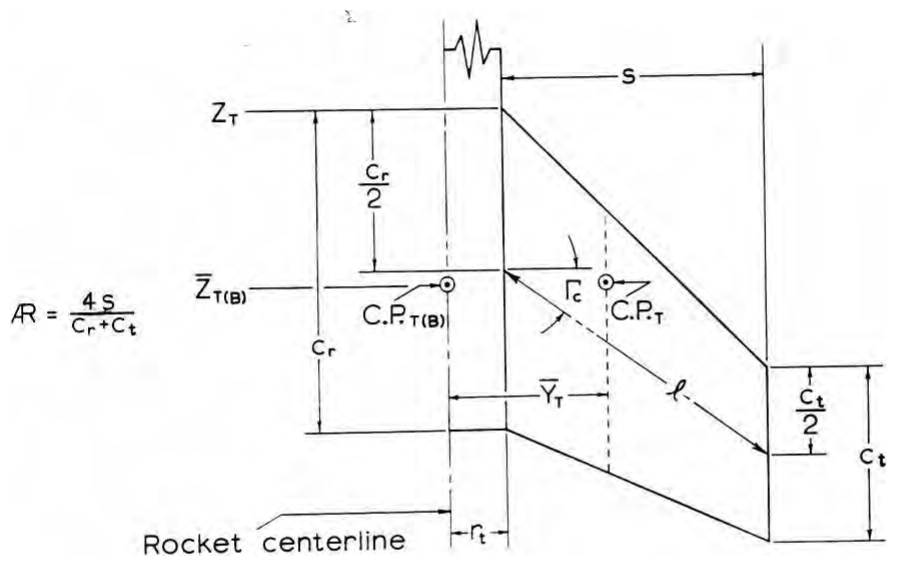
\includegraphics[width=0.75\textwidth,height=0.42\textheight,keepaspectratio]{figures/supplement/ch2-fig36-1994.png}
\end{center}

\noindent Figure 36: Notation used in determining the normal force curve slope
and center of pressure location of single fins and symmetrical fin assemblies.
$Z_T$ is the distance from the tip of the rocket's nose to the intersection of
the fin root and the fin leading edge. $\bar{Z}_{T(B)}$ is the distance from
the nose tip to the center of pressure of the fin assembly. $\ell$ is the
distance from the midpoint of the fin root chord to the midpoint of the fin tip
chord. The definition of $\AR$, the \emph{aspect ratio} of a pair of fins
joined at the root to create a ``wing'' of span $2s$, is also given.

\bigskip
\noindent\begin{minipage}{\linewidth}% keeps the 1973 figure with its note and caption
\edcap{The 1973 Figure 36, which this figure replaces:}

\begin{center}
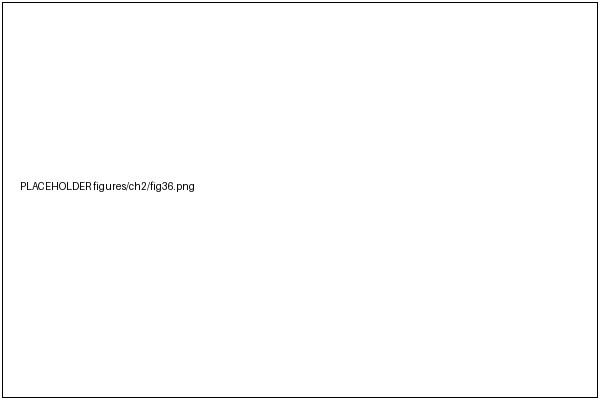
\includegraphics[width=0.6\textwidth,height=0.3\textheight,keepaspectratio]{figures/ch2/fig36.png}
\end{center}

Figure 36: Notation used in determining the normal force coefficient and center
of pressure location of single fins and symmetrical fin assemblies. $Z_T$ is the
distance from the tip of the nose to the intersection of the fin root and
leading edge; $\bar{Z}_{T(B)}$ is the distance from the nose tip to the center
of pressure of the fin assembly. The definition of $\AR$, the \emph{aspect
ratio} of a single fin, is also given.
\end{minipage}

\chapter{[Handwritten Corrections to Equations (115) Through (117)]}\label{supp:ch2-115-1994}

\noindent\edcap{This handwritten correction, which shows no author or date, is superseded by Mandell's
corrections of 15 February 2022, which come next. It is not applied in
Chapter~\ref{ch2}, which uses the 2022 text; its corrected equations agree with
the 2022 ones.}
\par\medskip

Equation~\eqref{ch2:eq:115} on page 251 should read
\begin{equation*}
\omega_Z = \frac{12\theta V A_f\bar{Y}_T k_r}{s c_r k_d\bigl[(1 + 3\lambda)s^{2} + 4(1 + 2\lambda)s r_t + 6(1 + \lambda)r_t^{2}\bigr]}
\end{equation*}

Note that $A_f$, the planform area of one fin, should appear in the numerator
rather than $A_r$, which in Barrowman analysis denotes the ``reference area''
and is defined as the cross-sectional area of the body at the base of the nose
cone (ref.\ pg.~187). $\bar{Y}_T$, $s$, $c_r$, and $r_t$ are illustrated in
Figure~\ref{ch2:fig:36} on page 194, along with the fin chord $c_t$ at the fin
tip. The value of $\bar{Y}_T$ is given by equation~\eqref{ch2:eq:90} on page
196 as
\begin{equation*}
\bar{Y}_T = r_t + \frac{s}{3}\left[\frac{c_r + 2c_t}{c_r + c_t}\right]
\end{equation*}
and $\lambda$ is given on page 253 as
\begin{equation*}
\lambda = \frac{c_t}{c_r}.
\end{equation*}

Aside from the error it contains, equation~\eqref{ch2:eq:115} could have (and
should have) been written in a more convenient form that does not give the
impression of an inverse dependence of $\omega_Z$ on $c_r$. Noting that
\begin{equation*}
A_f = s\left(\frac{c_r + c_t}{2}\right) = \frac{s c_r}{2}(1 + \lambda)
\end{equation*}
one can write equation~\eqref{ch2:eq:115} as
\begin{equation*}
\omega_Z = \frac{6\theta V\bar{Y}_T(1 + \lambda)k_r}{\bigl[(1 + 3\lambda)s^{2} + 4(1 + 2\lambda)s r_t + 6(1 + \lambda)r_t^{2}\bigr]k_d}
\end{equation*}

Equation~\eqref{ch2:eq:116} on page 253, which defines the roll forcing
interference coefficient $k_r$, also contains an error.
Equation~\eqref{ch2:eq:116} should read
\begin{multline*}
k_r = \frac{1}{\pi^{2}}\Biggl\{\frac{\pi^{2}}{4}\left(\frac{\tau + 1}{\tau}\right)^{2}
  + \frac{\pi}{\tau^{2}}\left(\frac{\tau^{2} + 1}{\tau - 1}\right)^{2}\arcsin\left(\frac{\tau^{2} - 1}{\tau^{2} + 1}\right)
  - \frac{2\pi}{\tau}\left(\frac{\tau + 1}{\tau - 1}\right)
  + \frac{8}{(\tau - 1)^{2}}\ln\left(\frac{\tau^{2} + 1}{2\tau}\right)\\
  + \left[\frac{\tau^{2} + 1}{\tau(\tau - 1)}\right]^{2}\left[\arcsin\left(\frac{\tau^{2} - 1}{\tau^{2} + 1}\right)\right]^{2}
  - \frac{4(\tau + 1)}{\tau(\tau - 1)}\arcsin\left(\frac{\tau^{2} - 1}{\tau^{2} + 1}\right)\Biggr\}
\end{multline*}

The error in the book consisted of omitting a superscript 2 in the second term.
The term given as
\begin{equation*}
\frac{\pi}{\tau^{2}}\left(\frac{\tau + 1}{\tau - 1}\right)^{2}\arcsin\left(\frac{\tau^{2} - 1}{\tau^{2} + 1}\right)
\end{equation*}
on page 253 should read
\begin{equation*}
\frac{\pi}{\tau^{2}}\left(\frac{\tau^{2} + 1}{\tau - 1}\right)^{2}\arcsin\left(\frac{\tau^{2} - 1}{\tau^{2} + 1}\right)
\end{equation*}
where
\begin{equation*}
\tau = \frac{s + r_t}{r_t}.
\end{equation*}

The roll damping interference coefficient $k_d$ is given correctly by
equation~\eqref{ch2:eq:117} on page 253 as
\begin{equation*}
k_d = 1 + \frac{\dfrac{\tau - \lambda}{\tau} - \dfrac{1 - \lambda}{\tau - 1}\ln\tau}{\dfrac{(\tau + 1)(\tau - \lambda)}{2} - \dfrac{(1 - \lambda)(\tau^{3} - 1)}{3(\tau - 1)}}
\end{equation*}
